% NOTES:
%   - Caching is the simplest client-side optimization that exploits past queries
%   - If sequences are realistic, cache hit rates should reflect sessions and refinement
%   - Goal is benchmark validation, not an exhaustive cache comparison

\begin{frame}{Validating the Benchmark: Client-side Caching}
    \begin{itemize}\setlength\itemsep{1em}
        \item Caching directly exploits data from past queries \parencite{hartig2011caching}
        \item Correlated query sequences should lead to cache hits
        \item Cache hit rates reveal whether our sequences behave as intended
        \item[$\Rightarrow$] Goal: validate the benchmark, not an exhaustive cache comparison
    \end{itemize}
\end{frame}

\begin{frame}{Caching Approaches}
    \centering
    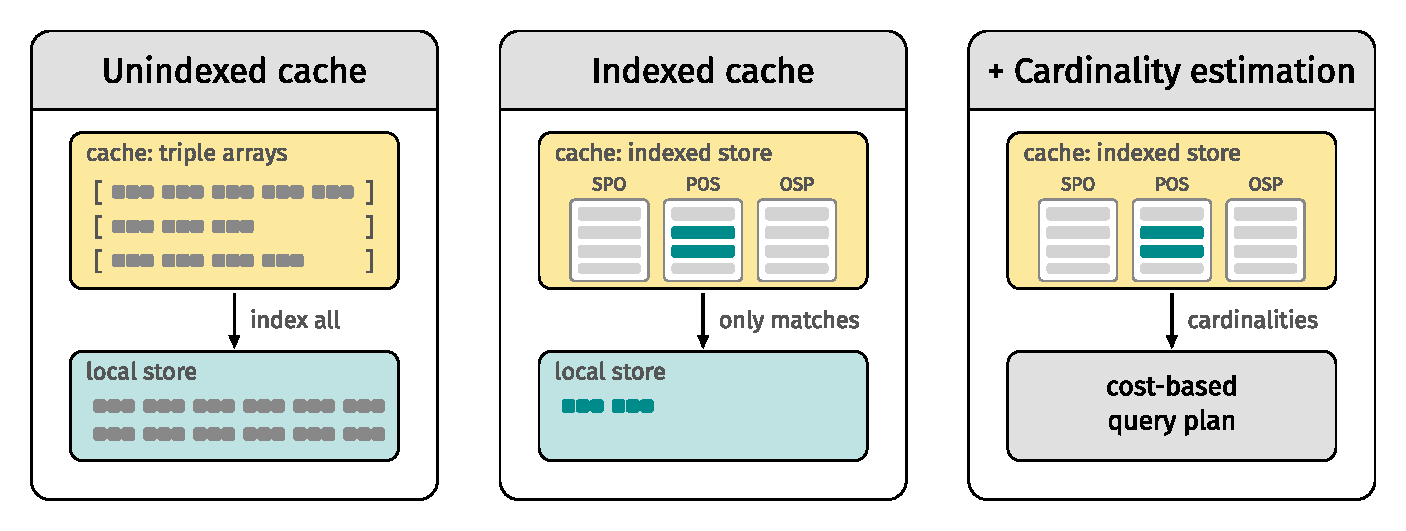
\includegraphics[width=\linewidth]{images/cache-approaches.pdf}

    \vspace{0.5em}
    Implemented in Comunica \parencite{taelman2018comunica}, LRU eviction, three sizes: S (350k quads, $\sim$10\%), M (700k, $\sim$20\%), L (1.4M, $\sim$40\%)
\end{frame}

\begin{frame}{Experimental Setup}
  \begin{block}{Workload}
    \begin{itemize}
        \item 8 generated sequences, 192 queries (discover and short templates)
    \end{itemize}
  \end{block}
  \begin{block}{Execution}
    \begin{itemize}
        \item Each sequence repeated 10 times, 70--90 ms injected network latency, 180 s timeout
        \item Cache scoped to a single sequence, no state shared between runs
    \end{itemize}
  \end{block}
  \begin{block}{Measured}
    \begin{itemize}
        \item Cache hit rates, evictions, and speedup over no cache
    \end{itemize}
  \end{block}
\end{frame}
